%%%%%%%%%%%%%%%%%%%%%%%%%%%%%%%%%%%%%%%%%
% Stylish Article
% LaTeX Template
% Version 2.2 (2020-10-22)
%
% This template has been downloaded from:
% http://www.LaTeXTemplates.com
%
% Original author:
% Mathias Legrand (legrand.mathias@gmail.com) 
% With extensive modifications by:
% Vel (vel@latextemplates.com)
%
% License:
% CC BY-NC-SA 3.0 (http://creativecommons.org/licenses/by-nc-sa/3.0/)
%
%%%%%%%%%%%%%%%%%%%%%%%%%%%%%%%%%%%%%%%%%

%----------------------------------------------------------------------------------------
%	PACKAGES AND OTHER DOCUMENT CONFIGURATIONS
%----------------------------------------------------------------------------------------

\documentclass[fleqn,10pt]{SelfArx} % Document font size and equations flushed left

\usepackage[english]{babel} % Specify a different language here - english by default
\usepackage{tabularx}
\usepackage{pdfpages}
\usepackage{graphicx}
\usepackage{lipsum} % Required to insert dummy text. To be removed otherwise

\newcommand{\aim}[2]{\textbf{Aim #1: #2}}
\newcommand{\aimOne}{\aim{1}}
\newcommand{\aimTwo}{\aim{2}}
\newcommand{\aimThree}{\aim{3}}
\newcommand{\aimFour}{\aim{4}}
\newcommand{\aimFive}{\aim{5}}
\newcommand{\GN}{{\textsc{GN}}}
%----------------------------------------------------------------------------------------
%	COLUMNS
%----------------------------------------------------------------------------------------

\setlength{\columnsep}{0.55cm} % Distance between the two columns of text
\setlength{\fboxrule}{0.75pt} % Width of the border around the abstract

%----------------------------------------------------------------------------------------
%	COLORS
%----------------------------------------------------------------------------------------

\definecolor{color1}{RGB}{0,0,90} % Color of the article title and sections
\definecolor{color2}{RGB}{0,20,20} % Color of the boxes behind the abstract and headings

%----------------------------------------------------------------------------------------
%	HYPERLINKS
%----------------------------------------------------------------------------------------

\usepackage{hyperref} % Required for hyperlinks

\hypersetup{
	hidelinks,
	colorlinks,
	breaklinks=true,
	urlcolor=color2,
	citecolor=color1,
	linkcolor=color1,
	bookmarksopen=false,
	pdftitle={Title},
	pdfauthor={Author},
}

%----------------------------------------------------------------------------------------
%	ARTICLE INFORMATION
%----------------------------------------------------------------------------------------

\JournalInfo{Solomon GGI Archives, Vol. I, No. 1, 1-5, 2023} % Journal information
\Archive{Supporting the Panorama Project} % Additional notes (e.g. copyright, DOI, review/research article)

\PaperTitle{Postdoc Proposal} % Article title

\Authors{Shelby Solomon Darnell\textsuperscript{1}} % Authors
%\Authors{Shelby Solomon Darnell\textsuperscript{1}*, James Smith\textsuperscript{2}} % Authors
\affiliation{\textsuperscript{1}\textit{Department of Genetics, Genomics and Informatics, UTHSC, Memphis, TN, United States of America}} % Author affiliation
%\affiliation{\textsuperscript{2}\textit{Department of Chemistry, University of Examples, London, United Kingdom}} % Author affiliation
\affiliation{*\textbf{Corresponding author}: shelby@shelbydarnell.com} % Corresponding author

\Keywords{Affective Genomics --- Computational pangenomics --- bespoke computing architecture --- Adaptive Artificial systems --- Causal inference} % Keywords - if you don't want any simply remove all the text between the curly brackets
\newcommand{\keywordname}{Keywords} % Defines the keywords heading name

%----------------------------------------------------------------------------------------
%	ABSTRACT
%----------------------------------------------------------------------------------------

%\Abstract{
%	GeneNetwork is an advanced systems genetics platform quickly evolving into a flagship NIH genetic database in functionality, usefulness, usability, and accessibility. As a postdoc, with a broad computer science background, working with seasoned researchers in genetics, genomics and informatics (GGI) there are several areas that must be worked on to aide the advancement of \GN\ while preparing to be a principle research investigator in GGI. In order to achieve this goal I will build new and augment existing functionality into \GN\ while participating in learning activities to shore up knowledge of genetics and genomics. 
%}

\Abstract{
	The Panorama project is an NSF funded large collaborative project that brings together computing hardware and software scientists and engineers to work on a bespoke hardware and software to better manage pangenomic computing. 
}

%----------------------------------------------------------------------------------------

\begin{document}

\maketitle % Output the title and abstract box

\tableofcontents % Output the contents section

\thispagestyle{empty} % Removes page numbering from the first page

%----------------------------------------------------------------------------------------
%	ARTICLE CONTENTS
%----------------------------------------------------------------------------------------

\section{Introduction}


\noindent Scholars world wide spend exhaustive amounts of time and effort reading, summarizing, converting, memorizing, and mixing knowledge for their own purposes, and to push science forward.
Since the inception of AI its promise has exponentially out-sized its capabilities; however, computing resources strong enough to exploit deep learning in conjunction with continual improvements in the use and management of `big data' have begun to close the gap between `perceived utility' and promise of AI.
`Perceived utility' is how the common person understands AIs use and helpfulness.
There are AI utilities, applications, and algorithms that are used widely for automation, recognition, navigation, semi-autonomous vehicles, mars rover exploration, deep question answering, and now creativity.
The essence of AI is getting computers to perform `intelligent' human tasks.
Pursuit of the same has caused some researchers to thoroughly examine and re-examine their definitions of intelligence.
Many see a humanoid android or automaton that is difficult to differentiate from a human as the pinnacle of AI; because AI as a field has so many areas in which it needs to improve to reach such a technical height, it is defined with many sub-fields.
The major sub-fields of AI include: machine learning, natural language processing, 
\cite{Azaria:2022} \cite{Zhang:2023} \cite{Foucart:2023} \cite{DePeau-Wilson:2023}

Since the deep learning boom in 2010, there has been a mad rush to apply and improve its techniques.
The first `killer' application was image classification, still and video.
Deep learning has made image classification so accurate until a large technology company has made it known that it has failed unless its `driverless' technology is the hallmark feature in its electric vehicles. 
Before the success of deep learning models on images classification attempts at `self-driving' vehicles failed or the idea was a `non-starter`.
As we tend to only hear about the most negative news, the existing Tesla `self-driving' cars are making moves on the road, mostly to the great delight of their owners.
Deep learning techniques have made the accuracy and error rate of many biometric technologies so enviable that many scientists consider some biometrics issues as solved, especially with modalities that are highly persistent, permanent and ubiquitous (e.g. iris, face, fingerprint).
As deep learning is being improved so goes the hardware used to run the necessary algorithms.

Consistently improving techniques and hardware leads to neural networks with billions of parameters instead of hundreds or thousands.
In the same vein, it seems that it takes a model with billions of parameters to really `understand' and respond using human language.

By training and painstakingly moderating humongous neural network modesl, OpenAI, was able to build what seems a quantum leap in the generative AI, ChatGPT a large language model that generates `mostly coherent' responses to human speech, without having anything close to a human curated script.
Although ChatGPT relies on a neural network model to accomplish its goals, it has popularized the term `large language model' (LLM).
In addition to creating a model that is magnificent at parsing information, understanding free-form human requests, and responding in a manner that can lead to the easy passing of the Turing test, OpenAI and others have trained neural network models on so many examples of data in different areas until `Generative AI' has pervaded the popular lexicon.
Generative AI (gAI) uses deep learning techniques to produce images, video, text, and more based on a free form query, making ChatGPT itself gAI.
Generative AI has recently gained attention due to the ability of services such as Midjourney (get ref) generating professional quality logos, portraits and other images based off of requests in free form human language.
The term `free form' is being used often as the generative models and LLMs do not need one to follow a script to generate output.

\begin{comment}
Thankfully AI is still an extremely hot topic; however, people are referring to everything that seems computationally smart as `artificial intelligence' (AI), mainly to keep things simple.
As stated in the introduction deep learning, mainly based on convolutional neural networks (CNNs), began showing breakthrough performance in image classification tasks, and scientists have been having a field day with the performance gains for multiple tasks, even in genomics [cite so many previous papers from the Diversity application write-up].
\end{comment}

%------------------------------------------------

\section{Appointment}
My appointment is with the University of Tennessee Health Sciences Center (UTHSC) in Memphis, Tennessee in the Genetic, Genomics, and Informatics group under the Panorama Project being done in conjunction with Christopher Batten at Cornell.
My direct mentors will be Associate Professor Pjotr Prins (UTHSC), Associate Professor Christopher Batten (Cornell) and Assistant Professor Erik Garrison (UTHSC).
The duration of the postdoc is up to two years, from April 2023 thru to end of March 2025.


%------------------------------------------------

\section{Strengths \& Weaknesses}\label{sec:weaknesses}

Science careers has a tool to aide young researchers in building an individual development plan, called
\hyperlink{https://myidp.sciencecareers.org}{myIDP}.

\subsection{Strong skills}
\begin{enumerate}[noitemsep]
    \item basic writing and editing
    \item writing for nonscientists
    \item speaking clearly and effectively
    \item presenting to nonscientists
    \item demonstrating workplace etiquette
    \item complying with rules and regulations
    \item maintaining positive relationships with colleauges
    \item providing instruction and guidance
    \item creating vision and goals
    \item serving as a role model
    \item careful recordkeeping practices
    \item understanding of data ownership/sharing issues
    \item demonstrating responsible authorship and publication practices
    \item demonstrating responsible conduct in human research
    \item how to maintain a professional network
    \item technical skills related to my specific research area
\end{enumerate}


\subsection{Improvement Approach}

\subsubsection{Areas for Improvement}
\begin{enumerate}[noitemsep]
    \item writing grant proposals
    \item developing/managing budgets
    \item delegating responsibilities
    \item planning and organizing projects
    \item how to negotiate
    \item contributing to institution (e.g. participate on committees)
    \item demonstrating responsible conduct in animal research
    \item statistical analysis
    \item seeking advice from advisors and mentors
    \item how to interview
    \item navigating the peer review process
\end{enumerate}



Write grant proposals for NSF Experiential Learning for Emerging and Novel Technologies (ExLENT) and the NIH Diversity Supplement opportunities.
Each will give experience with programs that target diverse populations and support investigations into artificial intelligence techniques.
In working on the preparation of these initial grant proposals, more than one area of improvement will be worked on, namely developing budgets, and planning projects.

Before writing the grant proposals research work must be completed up to a point of having published and presented some research work.
During the research I will work on seeking advice from advisors and mentors during the work, and learn how to better navigate the peer review process after submission of manuscripts.


Negotiation is another week point in my experience, to this end I will have to learn from my mentors negotiation tactics as I build my research team and interact with collaborators.

%One of the weakpoints listed in myIDP evaluation is that I have not demonstrated responsible conduct in animal research, that is because 
I find when uncomfortable friction appears in professional settings I do not negotiate the situation well, as in I copitulate to the aggressive party to avoid the friction.
I must learn how to navigate the friction and negotiate the best outcome for myself and my team, as the best outcome will push forward my major goals.
An activity I want to avoid, but should not -based on Pjotr's feedback- is planning/organizing events.
From my experience such an activity requires interacting with myriad types of personalities, many of whom I will have little common ground.
In order to become a well-known researcher I will be required to organize conferences, symposiums, research experience for undergraduates programs and more.
I will ask my mentors to be on the lookout for events I can help organize. 

This schedule includes learning activities, speaking engagements, research, writing, collaboration, and working on specific weak skills and deficiencies.
With this schedule mapped out to improve my overall research scientist qualities, the following list shows the main research thrusts of the postdoc.

\subsubsection{Training in Biology and Genomics}
\begin{description}
    \item[1. Scholarly Activities] The primary emphasis of this opportunity is to apply a comprehensive AI skillset and my diverse perspective to Panorama project. With Drs. Prins, Batten and Garrison serving as my mentors I will be guided properly as to developing solutions to meet the research requirements.
    \item[2. Educational Activities] New professors are encouraged to participate in seminars that help keep each other on the cutting edge of the field. As a computer scientist getting into genomics I will take several classes to enhance my skills. I will also attend the genomics seminar to keep abreast of the cutting edge in the field, while strengthening my core competencies.
    \item[3. Speaking Activities] There are many conferences in the field of genomics with artificial intelligence and data science tracks. Two upcoming such conferences with submissions due on July 31, 2023 are: the International Conference on Genetics and Genomics, the International Conference on Quantitative Genetics and Genomics (https://waset.org/quantitative-genetics-and-genomics-conference), and the International Conference on Computational Genomics and Evolution (https://waset.org/computational-genomics-and-evolution-conference). 
  \end{description}

Concerning the research component of the plan, three major aims will be 
\begin{enumerate}[noitemsep]
    \item Differential privacy algorithm development and testing
	\item[Aim] Aide in development of new pangenome layout algorithms
	\item[Aim] Support broader impact initiatives 
\end{enumerate} 

Each of these research components will be expounded upon in an upcoming section.

%\begin{description}
%	\item[Word] Definition
%	\item[Concept] Explanation
%	\item[Idea] Text
%\end{description}

%------------------------------------------------

\section{Background}\label{sec:background}

\subsection{Panorama Project}

The Panorama project is a five year NSF funded effort to create the first integrated rack scale acceleration paradigm specifically for computational pangenomics.
Christopher Batten and a team of seven primary investigators, including Pjotr Prins, currently lead this effort.

\subsubsection{Problem}
It has become necessary for computers to attempt analysis of massive datasets which need to be manipulated in irregular and rapidly changing ways while ensuring strict privacy guarantees.  
The ability to efficiently support large, sparse, dynamic yet private data for solving big complex problems on hetergeneous systems is one of the grand challenges in software/hardware systems research.
Addressing this grand challenge is the Panarama project by way of the exploration of integrated rack scale acceleration for computational genomics.
Integrated rack-scale acceleration refers to an emerging computer-systems paradigm that uses tens of tightly integrated computing nodes, each of which includes a mix of general-purpose processors and specialized accelerators interconnected with a special-purpose network. 
Computational pangenomics refers to a recent trend towards representing genomes, the genetic material of an organism, not as a single linear sequence of DNA base pairs but instead as an intricate network of sequences that efficiently represents the relationships between many individuals' genomes at once. 
Computational pangenomics naturally captures the trend towards big, sparse, dynamic, and private data and is thus a perfect application domain to explore heterogeneous software/hardware systems research. 

\subsubsection{Novelties}
The project's novelties are: a truly cross-stack approach spanning applications, programming languages, compilers, architecture, security, and privacy including use of a one-of-a-kind Panorama prototype system; new hardware techniques to accelerate domain-specific computing and to unify heterogeneous systems; new software techniques to let programmers harness the performance advantages of heterogeneous systems; and new software/hardware techniques to make such heterogeneous systems more secure.

\subsubsection{Impacts}
The project's impacts are: to specifically enable computational biologists to better see the ``genetic dark matter'' of population-wide genomics which has been to date hidden, opening up new scientific discoveries; and to more generally enable future computer users to more easily take advantage of heterogeneous computer systems to solve large and complex problems. 
This project is also pursuing two broader impact initiatives. 
The first is an ambitious yet concrete initiative to increase participation of under-represented minority students in computer science by developing a low-level computer-systems module for a new four-week summer program targeting rising sophomores. 
The second involves specific plans to grow the open-source software/hardware ecosystem in the computational-biology and computer-systems communities.

\subsubsection{Methods/Project Thrusts}
The Panorama project includes a highly interdisciplinary team of researchers across four focus areas: applications (computational biology), programming languages \& compilers, computer architecture, and security \& privacy. 
The team is taking a holistic software/hardware co-design approach to explore five tightly interconnected research thrusts. 
The first three thrusts are structured from top-down across the computing stack. 
Thrust 1 investigates new computational pangenomics data structures and algorithms and will develop PanoBench, a new benchmark suite suitable for driving the remaining thrusts. 
Thrust 2 investigates new programming-language and compiler techniques \cite{umar2022, xiang2022, hua2022mgx}. 
Thrust 3 investigates new computer architectures with support for a whole-rack manycore with 1M+ cores and a partitioned global address space, unified array-based accelerators, and application-specific accelerator chiplets for computational pangenomics. 
The final two thrusts cut across both software and hardware. 
Thrust 4 investigates new security and privacy techniques including scalable secure computation on heterogeneous rack-scale systems, secure rack-scale resource management with auto-tuning, and differential privacy and homomorphic encryption for pangenomics. 
Thrust 5 involves holistically evaluating the research ideas in the other thrusts through the use of a one-of-a-kind Panorama prototype system.


\subsection{Differential Privacy for Pangenomes}
We implement a differentially private haplotype sampling method in a pangenomics toolkit. It projects ϵ
-differentially private synthetic pangenome variation graphs out of pangenomes built from complete haplotype-resolved assemblies like those made in the Human Pangenome project. We generate ϵ
-differentially private graphs from the human major_histocompatibility_complex (MHC), and use these to explore the effects of algorithm paramaters on output.

Large medical cohorts with associations between genomes and phenotypes usually only provide controlled data access to trusted researchers. Our goal is to establish a standard whereby a they could release a fully-public transformation of this controlled data for global use by anyone. This would thus provide global biomedical utility without significant risk to study participants. We do so by applying tools from differential privacy.

Differential privacy is an approach to data release that which allows for the description of group characteristics without revealing information about single individuals. It quantifies privacy loss caused by the release of information, allowing us to reason about the risks that a particular data sharing model poses to individual privacy. We build on decades of work on differential privacy, which has yielded well-defined models of differentially private data publication [dwork2014]. Our work is similar to approaches that have been used for trajectory data release, but differs in the unique biomedical context and properties of the graph data structures we use. This has led to the need for an application-specific implementation.

Differential privacy provides tools that allow us to generate privacy-preserving synthetic databases out of real ones. We pursue this approach because we judge that it is easier to share static databases than organize access to differentially private queries. If we provide a tool to produce a differentially private synthetic pangenome, a genomics research project could release a pangenome that can be reused indefinitely by external researchers. Reuse of this database would not constitute increased privacy risk to individuals [dwork2014].


\section{Individual Development Plan}\label{sec:idp}
Shelby Solomon's individual development plan is based on the strengths and weaknesses listed in section~\ref{sec:weaknesses} and will build off of the background~\ref{sec:background}.

\subsection{Technical \& Research Aims}
\begin{description}
	\item[Aim 1] Create a specialized google-type gene-rank mechanism by ranking genes found in GWAS/QTL mapping using public data sources. 
	\item[Rationale] The point of gene-rank mechanism, at least the version most suitable to our aims, is to give researchers interesting sets of genes to study given a specific focus area.
For instance, when attempting to understand addiction the ability to both search over as many accessible sources as possible finding genes related to the topic and then being able to rank the `goodness' of the genes in a way that fits your `goodness' definition is a much desired tool for omics researchers.
Gunturkun\cite{Gunturkun:2022} et. al. have done the first part of this work at UTHSC with Pjotr Prins. 
They have developed \textit{Genecup}, a tool that mines for gene-keyword relationships from PubMed and the genome wide association studies catalogue\cite{Buniello:2019}.
Machine learning is used to disambiguate search topics, while the tool searches abstracts and finds genes with keywords together in the same sentence.
The tool builds an ontology to help support the searching of the databases, and upon fetching the information develops an interactive graph using the keywords, genes and articles it finds.
As the graph is interactive one can select nodes and investigate sentences from the abstracts that result from the user query.

Moving beyond this utility a gene-ranking mechnanism will be applied to the resultant genes listed with the returned results.
Why gene-ranking, because it can highlight genes and haplotypes -- a physical grouping of genomic variants that tend to be inherited together that typically reflects a unique combination of variants that reside near each other on a chromsome that can include a single or multiple genes \cite{NHGRI:Haplotype}.
We will quickly elaborate on some of the techniques before describing our methods.
	\item[Methods] One of the \GN\ innovative outcomes is to build a more powerful database system combining human and model organisms, where Mouse and rat will be combined in one data resource.
Data entry methods will undergo improvement by way of controlled vocabularies and ontologies to cover genotypes and phenotypes.
The improved database will use RDF+SPARQL which are technologies designed to make information on the web more interconnected and accessible.
Another added beauty of these technologies is that they are designed to speed up data access and querying, and most especially work optimally with AI tools.
Such linked data is explicitly encoded in a standardized machine-readable syntax with relations useful for machine learning exercises\cite{toh2019}.
Gene rank learner is a tool that will rely on data from multiple sources: pubmed, wikidata, \GN\, rat genome database (\href{http://rgd.mcw.edu}{RGD}), the gene expression omnibus (GEO)~\cite{NCBIGeo}, the search tool for the retrieval of interacting genes (STRING~\cite{STRING}), the database for annotation visualization and integrated discovery (DAVID~\cite{DAVID}), a new human gene database collected from volunteers~\cite{henderson2020}, and more.
One of the major aspects of this software will be a data management service that pulls ontologies, schema and other functional data information so that querying data from different sources is done transparently as if there is one large data source. 
In essence, creating a sort of data lake with bridges to different sources and an adaptive interface that supports quick addition of more data sources.
The initial algorithm implemented will be gene rank product used by Zeng et.al. in \cite{zeng2016discovering}, along with a function to count fold changes.
Correlation and consistency algorithms will be implemented next, as they take gene expression information into account, improving upon the significance of micro arrays (SAM) methods that would focus on gene expression yet were outperformed by gene rank product in the past.
An ant colony optimizer (ACO)~\cite{ACO:2009} will be implemented to traverse the large graph that will be created from the accumulation of data from the various sources.
ACO looks for optimal solutions using graph traversal; hence, we must define what we think to be a possible optimal set of interesting genes based off of a genes many characteristics.
Each of these algorithms will be compared against one another by being made available to the \GN\ community.
Those who use the gene rank learner will be encouraged to provide feedback.
Before being released to the \GN\ community we will provide multiple definitions of interesting genes, and compare the efficacy of the results from each technique.
This ensemble of algorithms will be implemented in the Julia programming language, some of the packages that will be used are \hyperlink{https://www.juliapackages.com/p/antcolony}{a package for using ant colony optimization -- antcolony}, \hyperlink{https://juliapackages.com/p/evolutionary}{a package for evolutionary computations -- evolutionary}, \hyperlink{https://juliapackages.com/p/mxnet}{a package to run ML algorithms with GPU optimization -- MXNet}, and the \hyperlink{https://alan-turing-institute.github.io/MLJ.jl/dev/}{a general ML framework -- MLJ}.
\end{description}

\begin{description}
	\item[Aim 2] Take human data collected by the BIG project and place it into a GeneNetwork clone database that is not fully open to the public due to the nature of human data ownership.
	\item[Concept] \GN\ is a systems genetic database whose development is funded by the NIH. As such it follows FAIR principles, uses open source software (OSS), and provides tools for researchers and citizen scientists alike. As \GN\ continues to progress it will be a flagship genetic database for the NIH given the effort and expertise brought to the fore concerning its development.
	\item[Idea] Shelby Solomon will use the most current source base for \GN\ which uses RDF+SPARQL for faster querying while connecting to multiple online sources. Upon setting up an empty version of \GN\ with the most up-to-date tools and code, including the Generank algorithm, the DNA sequences of the thousands of volunteers who have agreed to be part of the BIG project will be input. The system will then be hardened against unauthorized and authorized usage using secure logins, cryptography and possibly biometrics authentication.
\end{description}

\begin{description}
	\item[Aim 3] Begin an investigation into causality for understanding why diabetes affects blacks in a disproportionate manner, and how the situation can be improved.
	\item[Concept] Diabetes is unfortunately a prevalent illness that has an oversized effect on underrepresented American populations; including Natives, Blacks, and Mexican \cite{Winer:2004}. Diabetes can lead to renal (kidney) failure among many other live imperiling issues.
	\item[Idea] Based on a quick analysis of diabetes and its causes a causal diagram is presented in ~\ref{fig:diabetes-cm}. In thinking through a causal diagram for diabetes, because its complications lead to so many other serious issues in underrepresented communities, we need to look at causes that mediate and ones that are confounders.
 A list of causes that can be evaluated: damage to the pancreas, obesity, specific medicines, high cholesterol, age, family history and certain hormonal conditions/imbalances. 
 The following list are things that are not easily evaluated or known: genetic predisposition, genetic mutation, lifestyle, gestational complications, and chance.
In the causal diagram `genetic mutation', healthcare access, and lifestyle all connect to the outcome diabetes through mediators.
Mediators are like symptoms to a problem, while explaining a known subset of a cause a mediator does not encompass the full probability of a cause that effects a specific outcome.
Even with mediators the furthest causes from the outcome do not all have a direct line to the outcome in our diagram in order to make the diagram less confusing and complicated.
A much more simple diagram could have been created with three nodes with the two cause nodes representing the group of observable causes and the group of un-observable causes both having a direct connection to the diabetes outcome.
However, this oversimplification does not help with showing the minimal complexity for the onset of diabetes.
For instance, `genetic mutation' is un-observable, as is `genetic predisposition' while both being confounders.
Also when looking at the several mediators from `genetic mutation' I am using `genetic predisposition' as a catch all past the mutation, since there are three other mediators based off of that single cause.
These causes are Confounders because especially as combined with `family history' and `lifestyle' can be interchanged and swapped and reach the diabetes outcome, with high probability while also being able to `prevent' diabetes if any one is not attributable to an individual.
Then there are causes like `age' and `specific medicines' that can directly bring the onset of diabetes while not logically being able to be a lone catalyst for the same.
However, the diagram must be based off of our current knowledge and refined as we learn more, just like a machine learning model. 
\end{description}

\begin{description}
	\item[Aim] Differential privacy algorithm development and testing
	\item[Concept] To enable allowing a human pangenome graph to be constructed and publicly released using genome data from a diverse set of genome data by ensuring strong privacy for individuals.
	\item[Idea] Work with Garrison on securing individual and group data with DP algorithms and integrate into PanoBench.
\end{description}

\begin{description}
	\item[Aim] Aide in development of new pangenome layout algorithms
	\item[Concept] These layout algorithms can provide effective visualization that reveals the detailed structure of regions of the human pangenome, which were completely invisible to genomics researchers before.
	\item[Idea] Zhang and Garrison use stochastic gradient descent, a type of AI optimization with which I would love to experiment.
\end{description}

\begin{description}
	\item[Aim] Support broader impact initiatives 
	\item[Concept] All NSF grants must contain broader impact initiatives. This is due to the nature of work being funded by the taxpayer, it follows that projects should have as a partial focus `broader impacts' or aspects that further things that are `good for the people'.
	\item[Idea] I have participated in many `broader impacts' initiatives and guided many underrepresented students in the computing sciences, and look forward to supporting the same for the Panorama project by aiding in the mentoring and management of the low-level computer systems module for the 4-week summer program and support/grow the OSS ecosystem in computational biology.
\end{description}


\subsection{Postdoc timeline}
\captionsetup{font={scriptsize,sc,up,singlespacing}}
\begin{figure*}[h] % Figure at bottom of the page ([b] argument, could be "t" for top or "h" for here)
	\centering
	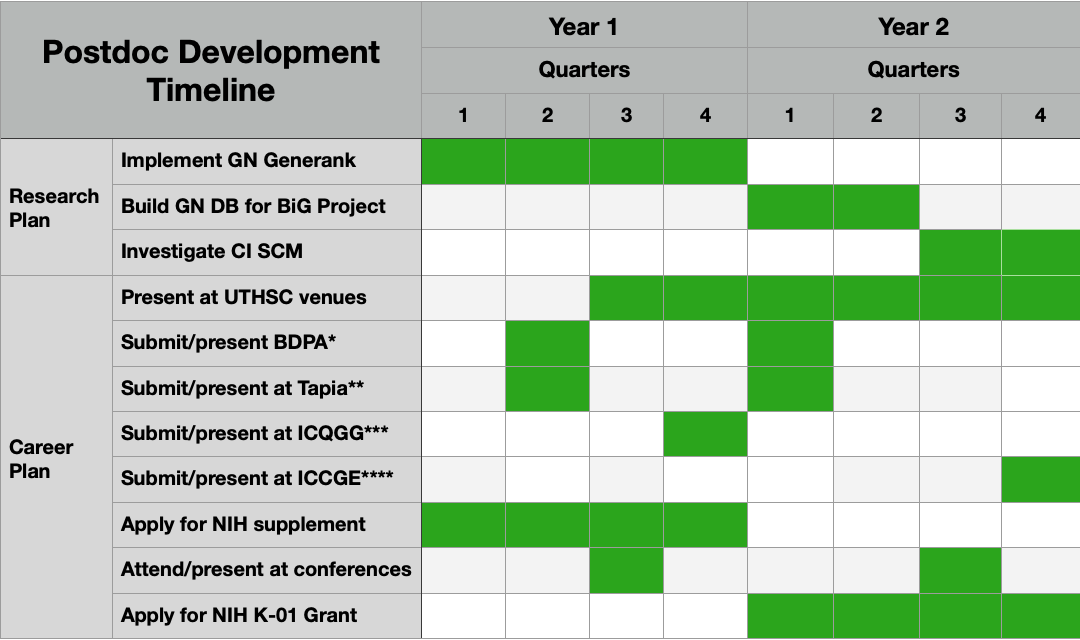
\includegraphics[width=\textwidth]{Figures/timeline-postdoc.eps}
	\caption{\textbf{Postdoc Timeline}\\
	* - Black Data Processing Associates, bdpa.org \\
	** - ACM/CMD-IT Tapia Celebration of Diversity in Computing\\
	*** - International Conference on Quantitative Genetics and Genomics\\
	**** - International Conference on Computational Genomics and Evolution
	}
	\label{fig:timeline}
\end{figure*}


%\includegraphics[width=0.4\textwidth, angle=0]{image1.pdf}


%\phantomsection
%\section*{Acknowledgments} % The \section*{} command stops section numbering

\addcontentsline{toc}{section}{Acknowledgments} % Adds this section to the table of contents

%So long and thanks for all the fish \cite{Figueredo:2009dg, Smith:2012qr}.

%----------------------------------------------------------------------------------------
%	REFERENCE LIST
%----------------------------------------------------------------------------------------
%\phantomsection
\newpage
\bibliographystyle{unsrt}
\bibliography{proposal.bib}

%----------------------------------------------------------------------------------------

\onecolumn
\appendix
%\section{Potential Courses}\label{sec:courses}
%\begin{table*}[ht]
\begin{table}[t]
\caption{Potential Courses}
\centering
\begin{tabular}{|p{0.3\linewidth}p{0.2\linewidth}|p{0.48\linewidth}|}
\hline
\textbf{TITLE} & \textbf{OFFERED BY} & \textbf{DESCRIPTION} \\ %&ISO numeric Code\\
\hline
\href{https://ocw.mit.edu/courses/15-075j-statistical-thinking-and-data-analysis-fall-2011/}{Statistical Thinking and Data Analysis} & MITOpenCourseware & Self explanatory \\
\hline
\href{https://ocw.mit.edu/courses/18-s997-high-dimensional-statistics-spring-2015/}{High-Dimensional Statistics} & MITOpenCourseware & Intro to the finite sample analysis of high-dimensional statistical methods, state-of-the-art regression, matrix estimation, and PCA. \\
\hline
Genetics, Genomics \& Informatics Seminar & UTHSC GGI & Discuss state-of-the-art research into genetics and genomics. \\
\hline
\href{https://catalog.uthsc.edu/preview_course_nopop.php?catoid=39&coid=64602}{Foundations of AI in Healthcare I} & UTHSC GGI & ID a biomedical/healthcare area of interest that may benefit from the application of AI/ML. \\
\hline
\href{https://catalog.uthsc.edu/preview_course_nopop.php?catoid=39&coid=64603}{Foundations of AI in Healthcare II} & UTHSC GGI & Explore modification and usage of ML algorithms.\\
\hline
Gene Structure and Function & UAH & Advanced studies of macromolecular structure and biological function of proteins and nucleic acids involved in the passage of genetic information and cellular response. Structural significance of viruses and molecular evolution included. \\
\hline
Biostatistics/AI & UAH with A\&M & \\
\hline
Psychobiology Stress \& Illness & UAH & Overview of physiological stress responses and their influence on health, behavior, and illness.\\
\hline
Bioinformatics I & UAH & Practical use in bioinformatics and X-ray crystallography \\
\hline
Bioinformatics II & UAH & Practical use in bioinformatics and applied genomics.\\
\hline
Microbial Genetics & UAH & Transmission, expression, and evolution of genes in microorganisms. Studies of chromosomes, plasmids, transposons, bacteriophages, and other genetic elements.\\
\hline
Advanced Molecular Techniques & UAH & Laboratory techniques in molecular biology including current methodology in genomics, proteomics, and RNA analysis.\\
\hline
Immunology & UAH & Innate, humoral, and cell-mediated immunity. Immune deficiencies and hypersensitivities. Autoimmunity, transplantation, and other genetic elements.\\
\hline
\end{tabular}
\end{table}

%\begin{table*}[ht]
\begin{table}[t]
\caption{Potential Courses}
\centering
\begin{tabular}{|p{0.3\linewidth}p{0.2\linewidth}|p{0.48\linewidth}|}
%\multicolumn{3}{|c|}{\textbf{Possible Courses}} \\
\hline
\textbf{TITLE} & \textbf{OFFERED BY} & \textbf{DESCRIPTION} \\ %&ISO numeric Code\\
\hline
Algorithms in Bioinformatics & UAB & This course introduces various fundamental algorithms and computational concepts for solving questions in bioinformatics and functional genomics. These include graph algorithms, dynamic programming, combinatorial algorithms, randomized algorithms, pattern matching, classification and clustering algorithms, hidden Markov models and more. Each concept will be introduced in the context of a concrete biological or genomic application. A broad range of topics will be covered, ranging from genome annotation, genome reconstruction, microarray data analysis, phylogeny reconstruction, sequence alignments, to variant detection. \\
\hline
Next-generation Sequencing Data Analysis & UAB & This course is aimed to equip participants with the essential knowledge and skills required to begin analyzing next-generation sequencing data and carry out some of the most common types of analysis. The topics covered in-depth during this course are the analysis of RNA-Seq, ChIP-Seq data, ATACseq data, and Single-cell data, with an optional Variant Calling session. The sessions will also include Introduction to next-generation sequencing (NGS) technologies, common NGS data analysis issues, applications of sequencing technologies, introduction to bioinformatics file formats (e.g. FASTQ, bam, bed) and bioinformatics toolkits. At the end of this course, participants will have the expertise to perform these data analysis independently.\\
\hline
Visual Analytics for Bioinformatics & UAB & We will cover representation of different data types, concentrating on those generated by data-rich platforms such as next-generation sequencing applications, flow/mass cytometry, and proteomics, and will discuss the use of visualization techniques applied to assessing data quality and troubleshooting. \\
\hline
\href{https://www.coursera.org/specializations/bioinformatics?action=enroll}{Bioinformatics specialization} & UC San Diego via Coursera & Master bioinformatics software and computational approaches in modern biology.\\
\hline
\end{tabular}
\end{table}

\end{document}